\input{../article_base.tex}
\title{פתרון מטלה 1 --- חישוביות וקוגניציה, 6119}

\usepackage{pgfplots}

% chktex-file 17
% chktex-file 9

\begin{document}
\maketitle
\maketitleprint[beige]

\section{שאלת הכנה}
נניח ש־$y : \RR^2 \to [2]$ המוגדר על־ידי $y(\bar{x}) = H(\bar{w} \cdot \bar{x})$ פרספטרון בינארי, נניח ש־$H = \indicator_{[0, \infty)}$.

\subquestion{}
נניח ש־$w_2 = 0$ וכן ש־$\bar{x} = {(7, 2)}^T$ אז $y(\bar{x}) = 0$, אז ננתח את תוצאת $\bar{z} = {(5, -10)}^T$.
\begin{solution}
	מתקיים $y(\bar{x}) = H(w_1 \cdot 7) = 0$ ולכן נסיק $w_1 < 0$, בהתאם נובע $y(\bar{x}) = H(5 \cdot w_1) = 0$.
\end{solution}

\subquestion{}
כאשר $\bar{w} = {(1, 1)}^T$ אז נמצא את $y^{-1}(\{ 1 \})$.
\begin{solution}
	נבחין כי מתקיים $y(\bar{x}) = 1 \iff H(\bar{w} \cdot \bar{x}) = 1 \iff 0 \le x_1 + x_2$ מהגדרה. \\
	כלומר כאשר $-x_1 \le x_2$.
\end{solution}

\subquestion{}
נניח ש־$\bar{x}, \bar{z} \in \RR^2$ דוגמות כך שמתקיים $\bar{w} \cdot \bar{x}, \bar{w} \cdot \bar{z} \ne 0$. \\
נבדוק מתי נקבל $y(\bar{x}) \ne y(\bar{z})$.
\begin{solution}
	כאשר הדוגמות מקיימות $\bar{x} = \alpha \bar{w}, \bar{z} = \beta \bar{w}$ עבור $\alpha, \beta > 0$ נקבל שהווקטורים תלויים לינארית ובפרט,
	\[
		H(\bar{w} \cdot \bar{x}) = 1
		\iff 0 \le \alpha {\lVert w \rVert}^2
		\iff 0 \le \beta {\lVert w \rVert}^2
		\iff H(\bar{w} \cdot \bar{z}) = 1
	\]
\end{solution}

\question{}
יהי $y = H(\bar{w} \cdot \bar{x})$ פרספטרון בינארי ותהיינה הדוגמות הבאות,
\[
	y^1 = 1, x^1 = {(2, 2)}^T,
	\quad
	y^2 = 1, x^2 = {(1, 3)}^T,
	\quad
	y^3 = 0, x^3 = {(-1, 0)}^T,
	\quad
	y^4 = 0, x^4 = {(-1, 2)}^T
\]

\subquestion{}
נניח ש־$\bar{w}^1 = {(1, 1)}^T$ ונצייר את הנקודות, את וקטור המשקולות ואת הישר המתאים.
נתאר את תהליך הלמידה של הפרספטרון בהתאם לדוגמות ואז נתאר את המצב החדש.
\begin{solution}
	נתחיל בתיאור:
	\begin{otherlanguage}{english}
		\begin{center}
			\begin{tikzpicture}
				\begin{axis}[ymin=-4,ymax=4,xmin=-4,xmax=4,samples=300,axis y line=middle,axis x line=middle]
					\addplot[mark=none] {-x};
					\node[label={180:{$x^1$}},circle,fill,inner sep=2pt] at (axis cs:2,2) {};
					\node[label={180:{$x^2$}},circle,fill,inner sep=2pt] at (axis cs:1,3) {};
					\node[label={180:{$x^3$}},circle,draw,inner sep=2pt] at (axis cs:-1,0) {};
					\node[label={180:{$x^4$}},circle,draw,inner sep=2pt] at (axis cs:-1,2) {};
					\node[label={180:{$w^1$}},inner sep=2pt] at (axis cs:1,1) {};
					\draw[->, >=stealth, thick] (axis cs:0,0) -- (axis cs:1,1);
				\end{axis}
			\end{tikzpicture}
		\end{center}
	\end{otherlanguage}
	נרצה להתחיל לבצע את תהליך הלמידה, ונבחין כי $H(w^1 x^1) = y^1 = y^2 = H(w^1 x^2)$ ולכן נדלג עליהם.
	נבצע את הליך הלמידה עם $\eta = 2$.
	נגיע למקרה $y^3 \ne H(w^1 x^3)$ ולכן נגדיר,
	\[
		w^2
		= w^1 + \eta (2y^3 - 1) x^3
		= {(1, 1)}^T + 2 (2 \cdot 0 - 1) {(-1, 0)}^T
		= {(3, 1)}^T
	\]
	נבדוק ונקבל $H(w^2 \cdot x^4) = y^4$ ולכן סיימנו את המעבר הראשון.
	נתחיל את המעבר השני ומחישוב ישיר נקבל $H(w^2 \cdot x^n) = y^n$ לכל $n \le 4$, כלומר סיימנו את הליך האימון.
	נתאר את המצב החדש:
	\begin{otherlanguage}{english}
		\begin{center}
			\begin{tikzpicture}
				\begin{axis}[ymin=-4,ymax=4,xmin=-4,xmax=4,samples=300,axis y line=middle,axis x line=middle]
					\addplot[mark=none] {-3 * x};
					\node[label={180:{$x^1$}},circle,fill,inner sep=2pt] at (axis cs:2,2) {};
					\node[label={180:{$x^2$}},circle,fill,inner sep=2pt] at (axis cs:1,3) {};
					\node[label={180:{$x^3$}},circle,draw,inner sep=2pt] at (axis cs:-1,0) {};
					\node[label={180:{$x^4$}},circle,draw,inner sep=2pt] at (axis cs:-1,2) {};
					\node[label={180:{$w^2$}},inner sep=2pt] at (axis cs:3,1) {};
					\draw[->, >=stealth, thick] (axis cs:0,0) -- (axis cs:3,1);
				\end{axis}
			\end{tikzpicture}
		\end{center}
	\end{otherlanguage}
	ונבחין כי גם גאומטרית הישר מסווג נכונה את הדוגמות.
\end{solution}

\subquestion{}
נניח ש־$w \in \RR^2$ וכן $y(x) = H(w \cdot x + T)$ פרספטרון בינארי עם סף. \\
בכל תת־סעיף נמצא ערכי $w, T$ עבורם מתקיימים התנאים הנתונים.

\subsubsection{i}
$y(x) = 1 \iff 2x_1 + x_2 > 0$.
\begin{solution}
	נגדיר אפריורית $T = 0, w = {(2, 1)}^T$ ונוכיח שהטענה מתקיימת. \\
	מתקיים,
	\[
		y(x) = 1
		\iff H(w \cdot x + T) > 0
		\iff 2x_1 + x_2 > 0
	\]
	כפי שרצינו.
\end{solution}

\subsubsection{ii}
$y = 1 \iff x_1 - 3x_2 < 4$.
\begin{solution}
	הפעם נגדיר $w = (1, -3)$ ו־$T = -4$ ונבחין כי,
	\[
		y(x) = 1
		\iff w \cdot x + T < 0
		\iff x_1 - 3x_2 < 4
	\]
	ומצאנו כי הטענה אכן מתקיימת.
\end{solution}

\subquestion{}
ידוע כי פרספטרון מבצע הפרדות לינאריות, אך נוכל להשתמש ברשת לביצוע הפרדות מעין זו. \\
נבנה רשת המקיימת $y = 1 \iff x_1 x_2 > 0$, כלומר רשת המסווגת תוכן על־ידי XNOR\@.
\begin{solution}
	נגדיר שלושה פרספטרונים בינאריים $y^k(x) : \RR^2 \to {\{0, 1\}}^2$ כאשר $k \in [2]$, המוגדרים על־ידי,
	\[
		w^1 = {(1, 0)}^T,
		\quad
		w^2 = {(0, 1)}^T
	\]
	עתה נגדיר את המשקל $w^3 = {(1, 1)}^T$ ונגדיר שכבה שנייה $y^3(x) = H(-w^3 x + \frac{1}{4})$ וכן $y^4(x) = H(w^3 x + \frac{3}{4})$, הם יהיו השכבה השנייה.
	לבסוף נגדיר את $y^5 = ({(1, 1)}^T \cdot x)$ בתור השכבה האחרונה.
	\begin{otherlanguage}{english}
		\begin{center}
			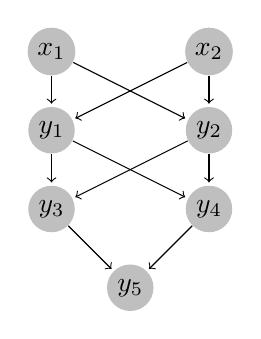
\begin{tikzpicture}[shorten >=1pt,->]
				\tikzstyle{vertex}=[circle,fill=black!25,minimum size=12pt,inner sep=2pt]
				\node[vertex] (x_1) at (-1,1) {$x_1$};
				\node[vertex] (x_2) at (1,1) {$x_2$};
				\node[vertex] (y_1) at (-1,0) {$y_1$};
				\node[vertex] (y_2) at (1,0) {$y_2$};
				\node[vertex] (y_3) at (-1,-1) {$y_3$};
				\node[vertex] (y_4) at (1,-1) {$y_4$};
				\node[vertex] (y_5) at (0,-2) {$y_5$};
				\draw (x_1) -> (y_1);
				\draw (x_2) -> (y_1);
				\draw (x_1) -> (y_2);
				\draw (x_2) -> (y_2);
				\draw (y_1) -> (y_3);
				\draw (y_2) -> (y_3);
				\draw (y_1) -> (y_4);
				\draw (y_2) -> (y_4);
				\draw (y_3) -> (y_5);
				\draw (y_4) -> (y_5);
			\end{tikzpicture}
		\end{center}
	\end{otherlanguage}
	נעבור להוכחה שהרשת אכן עובדת.
	\begin{proof}
		יהי $x = {(x_1, x_2)}^T$, אז נקבל $(y^1, y^2)(x) = {(H(x_1), H(x_2))}^2$.
		כלומר עתה נוכל להניח שהשכבה הראשונה לא קיימת אך ש־$x \in {\{0, 1\}}^2$.
		נבחין כי $y^3(x) = 1 \iff \frac{1}{4} > x^1 + x^2 \iff x^1 = x^2 = 0$, באופן דומה נקבל ש־$y^4(x) = 1 \iff x^1 = x^2 = 1$.
		לבסוף $(y^5 \circ (y^3, y^4))(x) = 1 \iff y^3(x) + y^4(x) > 0 \iff (x^1 = x^2 = 1) \lor (x^1 = x^2 = 0)$
	\end{proof}
\end{solution}

\end{document}
